\chapter{Introduction to NetKAT}

Software Defined Networking, or SDN, is a huge paradigm shift in the computing world.  
Traditional networking involves 
expensive, proprietary "boxes" from major vendors, plugging them in, configuring them, and hoping they 
meet your needs.  
But traditional networking suffers from these maladies:

\begin{itemize}
\item The devices are flexible only within narrow configuration parameters. 
Special requirements, like preventing certain kinds of devices from mobility, or configuring 
the spanning tree to prefer certain paths, are either impossible or expensive.
\item While the devices are powered by software, there's no workable way to examine the underlying code or prove it's correct.  
\item Upgrades tend to be the forklift-variety, since mixing and matching old and new hardware is a dicey proposition
\ldots not to mention mixing hardware from different vendors.
\item Configuration is not easily automated. 
Solutions are often proprietary, require special programming languages, and are not interchangeable.
Because of this, modern data center virtualization is more difficult.
\item Adding support for new protocols is slow and expensive.
\end{itemize}

With SDN, data centers can step off the proprietary network treadmill.  
Its a shift similar to the personal computer revolution of the 1980's.
Before that, IBM and similar mainframes controlled the computer space, and required the same kinds of 
forklift upgrades networks do.
The IBM Personal Computer opened up the architecture to competitors, who could then design and build extensions
that made it more useful.
This created a snowball effect, with hardware extensions like the mouse and Ethernet cards opening the way 
for new software like Microsoft Windows and the Netscape browser.

SDN opens network devices in a similar manner, allowing them to be extended and manipulated in interesting,
user-defined ways.
Although the term SDN has been hijacked to mean many things, it most often refers to OpenFlow-enabled 
network software and devices.
OpenFlow is an open protocol defined by the Open Network Foundation that manipulates the control 
plane of a network intermediary.  

Frenetic is an OpenFlow controller, meaning it talks the OpenFlow protocol to network intermediaries.  
In turn, it exposes an API that can be used to write network programs easily.
It works with any network intermediary that understands the OpenFlow 1.0 protocol -- 
both hardware devices like the HP 2920 and software ``devices'' like Open vSwitch.  
So let's take a brief look at OpenFlow itself.

\section{Introduction to OpenFlow}

Every network device -- from the lowliest repeater, to firewalls and load balancers, all the way up to the most complex router -- has two conceptual layers:

\begin{description}
\item[The data plane] performs actions on packets.   
It manipulates headers, copies packets to outgoing (or egress) ports, or drops packets.
It consults control tables - MAC address tables, ARP caches, OSPF tables, etc. - to guide it.  
\item[The control plane] manipulates the control tables themselves.
People, in turn, may manipulate the control plane through configuration software.
Or packets may do it: specialized ones like OSPF neighbor exchange, ARP requests, or just examining plain ol'
packets themselves.
But they never actually touch the packets.
\end{description}

This separation is only conceptual.
You'd be hard pressed to open a network device, point to a chip and say, "That's the data plane."
It helps in understanding a device, though, because they have different goals:

\begin{description}
\item[The data plane]'s job is to move data as quickly as possible.
It relies more on fast table lookups than complex algorithms.
\item[The control plane] works more flexibly, yet conservatively.
Control tables should not change often, and when they do, appropriate checks and balances should be applied to
ensure the data plane keeps working.  
For example, the Spanning Tree Protocol (or STP) ensures packets are routed along the shortest path with no
loops.  
Calculating the spanning tree is the control plane's job, as its complex. 
But once that's calculated, the data plane can use it to forward packets quickly.
\end{description}

A traditional network device looks like this. 
The control plane is closed and contained fully within the box.

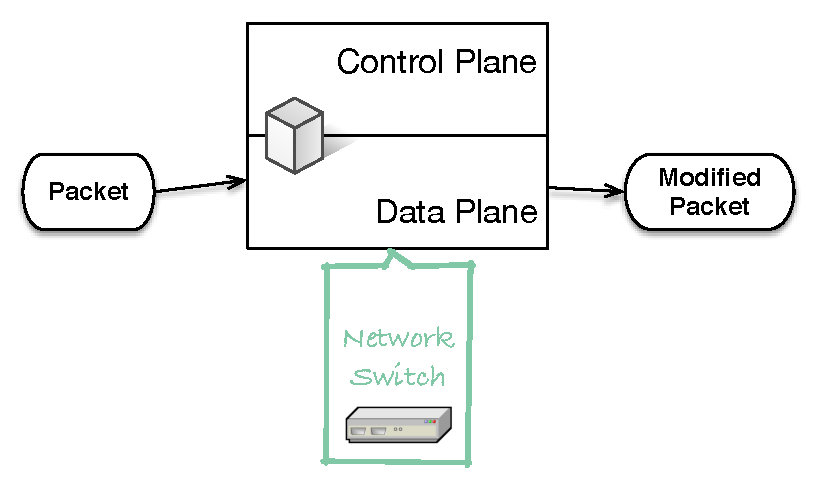
\includegraphics{traditional_device_planes}

The OpenFlow protocol makes the control plane \textit{programmable}.
Rather than relying on the entire program being inside the box, you write a program that advises the control plane
and runs outside the box.
It's like an advisor that makes aribtrarily complex control table manipulations.  
The programmable piece runs on any standard computer, and is collectively called the \textit{controller}.  

DIAGRAM HERE

The controller can be written in any language and run on any computer \ldots the only requirement is it must speak the
OpenFlow protocol to the device.  
You can think of these two pieces working in a tandem through an OpenFlow conversation:

\begin{description}
\item[Device:] I don't know what to do with this packet.  It came in port 3 from Ethernet mac address 10:23:10:59:12:fb:5c.
\item[Controller:] OK.  I'll memorize it.  In the meantime, send it out all ports on the switch except port 3.  
\item[Device:] I don't know what to do with this packet.  It's bound for Ethernet mac address 10:23:10:59:12:fb:5c.
\item[Controller:]  Oh yeah.  I know that's on port 3.  Install a rule so all packets going to that mac address go out port 3.
\item[Device:] OK!
\item[Controller:] How many packets have went out port 3, by the way?
\item[Device:] 82,120.
\item[Device:] (To itself) I just saw a packet destined for Ethernet mac address 10:23:10:59:12:fb:5c, but I have a rule for dealing with it.  I'm gonna send it out port 3.  
\end{description}

OpenFlow boils down control plane functionality to a common core, and many of the decisions can be made there.
Any complex decisions that can't be handled independently by the control plane can be offloaded to the controller.  
In a well-designed Software Defined Network, the controller gets involved only when necessary.
After all, the conversation between the device and the controller takes time, and anything that can 
eliminate this conversation makes the packets go faster.

So, central to the OpenFlow model is the \textit{flow table}.  
Flow tables have \textit{entries}, sometimes called \textit{flow rules}, that are consulted for making decisions.
A sample flow table might look like this:

DIAGRAM HERE

What's possible in a flow entry?
There's a lot of flexibility here:

\begin{description}
\item[A match] specifies patterns of packet header and metadata values.
OpenFlow 1.3 defines 40 different fields to match: some popular ones are the Input Port, 
the Ethernet Destination mac address, and the TCP destination port.
The match values can either be exact (like 10:23:10:59:12:fb:5c above) or wild carded (like 128.56.0.0/16 for a
particular Ip subnet).
\item[An instruction] tells what to do if the match occurs.  
Instructions can apply actions (send a packet out a port, or write some header information, 
or send a packet to the controller), 
invoke groups (like a function call in a programming language), or set variables.
\item[A priority] defines the order that matches are consulted.  
When more than one entry matches a particular packet, the entry with the highest priority wins.
\item[A cookie] is a primary key for an entry.
The cookie value means nothing to the device, but the controller can use it to delete or modify entries later.
\end{description}

In our example above, the controller installed a flow entry matching Ethernet Destination 10:23:10:59:12:fb:5c, 
and an instruction applying the action "Output it through Port 3".

OpenFlow's flow table model is \textit{abstract}.
An OpenFlow device is not necessarily going to find a RAM chip with the matches, 
instructions and priorities \ldots although a pure software switch like Open vSwitch might mirror it quite closely.
Instead, the controller asks the device to install entries, and the device accommodates it by placing entries in its
own tables.
For example, a real network device might have an L3 table that matches subnets with the various ports that have
IP gateways.
A programmer, knowing this table exists, can write instructions that match on those ports, and place it directly in the
table accordingly.

Suppose you wanted to write your own controller from scratch.  
You could do that just by talking the OpenFlow protocol.
Let's say you wrote this program in Node.js and placed it on the server "controller.example.com", 
listening on TCP port 6653.
Then you'd just point your OpenFlow network device at controller.example.com:6653.
Then your program could install flow table entries into the network device over the OpenFlow protocol.

Hmmm.
Sounds pretty easy, but \ldots

\section{OpenFlow is Difficult}

\subsection{OpenFlow Tables Are Difficult to Program}

Writing flow table entries directly is like writing programs in assembly language.

\subsection{OpenFlow Tables Are Difficult to Compose}

\section{NetKAT Makes Network Programming Easier}

\section{Predicates}

A NetKAT \textit{predicate} is a clause used to match packets.
The base language is pretty straightforward:

\bigskip
\begin{tabularx}{6in}{|c|X|}
\hline\hline
SwitchEq($n$) & Matches packets that arrive on switch $n$, where $n$ is the Datapath ID of the switch.  
\\ \hline
PortEq($n$) & Matches packets that arrive on port $n$.  Generally ports are numbered 1-$m$, where $m$ is the
number of interfaces, but they don't need to be consecutive.  
\\ \hline
EthSrcEq($mac$) & Matches packets whose Ethernet Mac source address is $mac$, which is a string in the standard form $nn:nn:nn:nn:nn:nn$ where the $n$'s are lowercase hexadecimal digits.
\\ \hline
EthDstEq($mac$) & Matches packets whose Ethernet Mac destination address is $mac$.
\\ \hline
VlanEq($vlan$) & Matches packets whose VLAN is $vlan$, and integer from 1-4096.  Packets without a VLAN are never matched by this predicate.
\\ \hline
VlanPcpEq($p$) & Matches packets whose VLAN Priority Code Point is $p$.  Packets without a VLAN are never matched by this predicate.
\\ \hline
EthTypeEq($t$) & Matches packets whose Ethernet Type is $t$, where t is a 32 bit integer.  Popular values of $t$ are 0x800 for IP and 0x806 for ARP.  
\\ \hline
IPProtoEq($p$) & Matches packets whose IP Protocol is $p$, a number from 0-255.  
Popular values are 1 for ICMP, 6 for TCP and 17 for UDP.  
This match only makes sense when EthTypeEq([0x800, 0x806]) (IP or ARP). 
\\ \hline
IPSrcEq($addr$, $mask$) & Matches packets whose IP source address is $addr$.  
If $mask$ is provided, a number from 1-32, this matches all hosts on a network whose first $mask$ bits match the host.
If it's omitted, the entire address is matched -- i.e. only one IP host.  
This match only makes sense when EthTypeEq([0x800, 0x806]) (IP or ARP). 
\\ \hline
IPDstEq($addr$, $mask$) & Matches packets whose IP destination address is $addr$.  
Follows same rules as IpSrcEq.
\\ \hline
TCPSrcPortEq($p$) & Matches packets whose TCP source port is $p$, an integer from 0-65535.
\\ \hline
TCPDstPortEq($p$) & Matches packets whose TCP destination port is $p$, an integer from 0-65535.
Popular values are 80 for HTTP, 22 for SSH, and 443 for SSL.  
\end{tabularx}

If you're familiar with OpenFlow, this list should look familiar to you -- it's exactly the same list of fields you can 
use in an OpenFlow flow table. 
NetKAT, however, augments these matching rules with combination operators:

\bigskip
\begin{tabularx}{4in}{|c|X|}
\hline\hline
$p1$ \& $p2$ & Matches packets that satisfy $p1$ AND $p2$
\\ \hline  
And($p1$, $p2$, \ldots, $pn$) & Matches packets that satisfy all the predicates: $p1$ AND $p2$ AND \ldots AND $pn$
\\ \hline  
$p1$ TODO $p2$ & Matches packets that satisfy $p1$ OR $p2$
\\ \hline  
Or($p1$, $p2$, \ldots, $pn$) & Matches packets that satisfy one of the predicates: $p1$ OR $p2$ OR \ldots OR $pn$
\end{tabularx}


\section{Policies}

\section{Events and Hooks}

